\documentclass{beamer}
%[aspectratio=169]   \usepackage[czech]{babel}
\usepackage{apo-lecture}
\usepackage{pdfpages}
\usepackage{pdfcomment}
\usepackage{listings}
\usepackage{array,multirow}

\subtitle{Lekce 02. Reprezentace čísel}
\author{Petr Štěpán\\ \small\texttt{stepan@fel.cvut.cz}}
\begin{document}

\maketitle

\section{Operace s celými čísly}

\begin{frame}
\frametitle{Opakování}
V minulé lekci jsme měli:
\begin{itemize}
\item Reprezentace bitu pomocí napětí
\item Reprezentace bajtů jako více paralelních vodičů, každý s hodnotou jednoho bitu
\item Sčítání dvou celých kladných čísel
\item Posun celých čísel (násobení, nebo dělení mocninou 2)
\end{itemize}

Dnes:
\begin{itemize}
\item Rozsahy celých čísel a ukládání do paměti
\item Násobení a dělení celých kladných čísel 
\item Reprezentace záporných čísel a operace s nimi
\item Přetečení sčítání a odčítání
\item Reálná čísla
\end{itemize}

\end{frame}


\begin{frame}
\frametitle{Kladná čísla}
Reprezentace celých kladných čísel

V jazyce C jsou typy (podle normy ISO/IEC 9899:TC3):
\begin{tabular}{|l|r|r|c|}\hline
typ & min & max & počet bajtů\\ \hline
unsigned char & 0 & 255 & 1 \\ \hline
unsigned short & 0 & 65 535 & 2 \\ \hline 
unsigned long & 0 & 4 294 967 295 & 4 \\ \hline
unsigned long long & 0 & 18 446 744 073 709 551 615 & 8 \\ \hline
\end{tabular}

\begin{itemize}
\item Norma není vždy dodržována, \texttt{unsigned int} by měl mít jen 2 bajty, ale většinou má 4 bajty (GNU, MS C).
\item Pokud chcete mít jistotu, musíte si pro cílovou platformu zjistit rozsah pomocí příkazu např. \texttt{sizeof(int)}
\end{itemize}

\end{frame}


\begin{frame}
\frametitle{Kladná čísla}
V zápis konstant v jazyce C v soustavě:
\begin{itemize}
\item desítkové -- nesmí začínat 0 kromě 0
\item osmičkové -- začíná 0
\item hexadecimální -- začíná 0x
\item binární -- začíná 0b (pouze GNU překladač)
\end{itemize}
\bigskip
Příklad: 252 == 0xfc == 0374 == 0b11111100
\bigskip

Poznámka: Podle hexadecimálního zápisu zjistíte velikost čísla v bajtech, např. 0x123456 se vejde do tří bajtů.
\end{frame}


\begin{frame}
\frametitle{Kladná čísla - uložení v paměti}

\begin{itemize}
\item Paměť počítače pracuje s bajty
\item Historicky vzniklo několik možností uložení čísel do paměti.
\end{itemize}

Jak lze tedy uložit číslo 0x12345678 do paměti:
\begin{tabular}{|c|c|c|}\hline
adresa & Big-endian & Little-endian \\ \hline
400 & 0x12 & 0x78 \\ \hline
401 & 0x34 & 0x56 \\ \hline
402 & 0x56 & 0x34 \\ \hline
403 & 0x78 & 0x12 \\ \hline
\end{tabular}

\begin{itemize}
\item Procesory Intel zavedly little-endian, procesory Motorola zavedly big-endian.
\item Je to důležité, když získáte například přes internet data po bajtech, musíte definovat, jaká čísla reprezentují
\item RISC V - little-endian, MIPS - big-endian
\item Bitcoin - DER signatures big-endian, transaction hash little-endian
\end{itemize}
\end{frame}

\begin{frame}[fragile]
\frametitle{Kladná čísla - kvíz}
\begin{minted}{c}
#include <stdio.h>
int main() {
  unsigned char p[] = {0,0,0,0};
  *(int*)p=10;
  printf("%02x,%02x,%02x,%02x\n", p[0],p[1],p[2],p[3]);
}
\end{minted}

Co bude výstupem tohoto programu na procesorech Intel?
\begin{itemize}
\item[A] nic, program nelze přeložit
\item[B] náhodný výstup, p  nelze přetypovat na *int
\item[C] 0a,00,00,00 
\item[D] 00,00,00,0a
\end{itemize}
\end{frame}



\begin{frame}
\frametitle{Násobení celých čísel}

Stejný princip násobení, jak jste se ho naučili na základní škole pro desítkovou soustavu:
\begin{columns}
\begin{column}{0.4\textwidth}
\texttt{\phantom{xxx}153}\\
\texttt{\phantom{xxx}*45}\\
\vspace{-8pt}
\rule[0pt]{1.5cm}{0.1pt}\\
\texttt{\phantom{xxx}765}\\
\texttt{\phantom{xx}612 }\\
\vspace{-8pt}
\rule[0pt]{1.5cm}{0.1pt}\\
\texttt{\phantom{xx}6885}\\
\end{column}
\hfill
\begin{column}{0.4\textwidth}
\texttt{\phantom{xxxxxx}10011001}\\
\texttt{\phantom{xxxxxxx}*101101}\\
\vspace{-8pt}
\rule[0pt]{3cm}{0.4pt}\\
\texttt{\phantom{xxxxxx}10011001}\\
\texttt{\phantom{xxxxx}00000000}\\
\texttt{\phantom{xxxx}10011001}\\
\texttt{\phantom{xxx}10011001}\\
\texttt{\phantom{xx}00000000}\\
\texttt{\phantom{x}10011001}\\
\vspace{-8pt}
\rule[0pt]{3cm}{0.4pt}\\
\texttt{\phantom{x}1101011100101}\\
\end{column}
\end{columns}

\end{frame}

\begin{frame}
\frametitle{Násobení celých čísel}

Podle uvedeného algoritmu můžeme vytvořit náseldující násobičku s posuvným registrem:\\
(A,B 32 bitů, výsledek 64 bitů)
\begin{center}
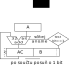
\includegraphics[width=0.45\textwidth]{multiplier-seq.pdf}
\end{center}
\begin{itemize}
\item Výsledek je ve dvou registrech AC a B 
\item Pomalé, už sčítání je náročné, nyní 32 nebo 64 sčítání.
\end{itemize}
\end{frame}


\begin{frame}
\frametitle{Rychlé násobení - Wallace tree}

Jak to zrychlit - odložené carry (Carry Save Adder).\\
Jak nejrychleji spočítat součet čtyř 32-bitových čísel:\\
\begin{columns}
\begin{column}{0.35\textwidth}
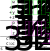
\includegraphics[width=1.0\textwidth]{wallace-tree.pdf}
\end{column}
\hfill
\begin{column}{0.65\textwidth}
\begin{itemize}
\item Sečteme paralelně p=w+x a q=y+z a potom p+q -- trvá dlouho, nejméně doby dvou plných součtů
\item Odložíme carry (nebudeme carry propagovat, jen v posledním kroku):
\begin{itemize}
\item 1. krok použijeme Full adder a sečteme vždy bity $w_i+x_i+y_i = c'_ip_i$
\item 2. krok použijeme Full adder a sečteme vždy bity $p_i+c'_{i-1}+z_i = c_iq_i$
\item 3. krok použijeme normální sčítačku 32-bitových čísel ($s_0=q_0$, $c'_32$ připojíme ke $q$)
\end{itemize}
\end{itemize}
\end{column}
\end{columns}
\end{frame}

\begin{frame}
\frametitle{Rychlé násobení - Wallace tree}

Použijeme předchozí princip na co nejrychlejší součet 32 nebo 64 různých čísel:
\begin{columns}
\begin{column}{0.6\textwidth}
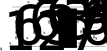
\includegraphics[width=1.0\textwidth]{wallace-tree2.pdf}
\end{column}
\hfill
\begin{column}{0.4\textwidth}
\begin{itemize}
\item Součiny jsou jednoduché: $x_iy_j=x_i$~\texttt{and}~$y_j$
\item Nejtěžší je sečíst prostřední sloupec 64 jednobitových čísel
\item Pustíme na všechny bity co můžeme paralelně sčítačky a carry budeme přičítat v dalších krocích
\item V první fázi to bude 1323 sčítaček
\end{itemize}
\end{column}
\end{columns}

\end{frame}

\begin{frame}[shrink=5]
\frametitle{Rychlé násobení - Wallace tree}

Když se podíváme jen na prostřední nejdelší sloupec:
\begin{center}
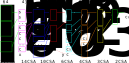
\includegraphics[width=0.8\textwidth]{wallace-tree3.pdf}
\end{center}

\begin{itemize}
\item Vydíme, že za 8 kroků sčítaček, tedy 16 zpoždění hradel nám zbývá sečíst dva bity
\item Vpravo od tohoto sloupce je již vše sečteno a již se i propagovali všechny carry
\item Zbývá sečíst dvě 64-bitová čísla (součty a carry), což se dá stihnout také za 16 zpoždění hradel
\item Výsledek - vynásobíme dvě čísla za cenu doby odpovídající dvou součtům
\end{itemize}

\end{frame}


\begin{frame}
\frametitle{Dělení celých čísel}

Dělení lze zkonstruovat podobně, jako jste se učili na základní škole:
\bigskip
\begin{columns}
\begin{column}{0.4\textwidth}
\texttt{\phantom{-}240:11=21}\\
\texttt{-22}\\
\vspace{-8pt}
\rule[0pt]{1cm}{0.1pt}\\
\texttt{\phantom{xx}20}\\
\texttt{\phantom{x}-11}\\
\vspace{-8pt}
\rule[0pt]{1cm}{0.1pt}\\
\texttt{\phantom{xxx}9}\\
\end{column}
\hfill
\begin{column}{0.4\textwidth}
\texttt{\phantom{x}11110000:1011=10101}\\
\texttt{-1011}\\
\vspace{-8pt}
\rule[0pt]{1cm}{0.4pt}\\
\texttt{\phantom{xx}1000}\\
\texttt{\phantom{xx}10000}\\
\texttt{\phantom{xx}-1011}\\
\vspace{-8pt}
\rule[0pt]{1.4cm}{0.4pt}\\
\texttt{\phantom{xxxx}1010}\\
\texttt{\phantom{xxxx}10100}\\
\texttt{\phantom{xxxx}-1011}\\
\vspace{-8pt}
\rule[0pt]{1.8cm}{0.4pt}\\
\texttt{\phantom{xxxxx}1001}\\
\end{column}
\end{columns}
\bigskip
Oba výpočty počítají, že 240 děleno 11 je 21 a zbytek neboli \texttt{240\%11=9}.

\end{frame}


\begin{frame}
\frametitle{Dělení celých čísel}

Dělička počítající \texttt{A/B}, A má 64 bitů, B 32 bitů:\\
\begin{columns}
\begin{column}{0.4\textwidth}
číslo A je uloženo ve dvou registrech AC,A\\¨
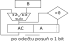
\includegraphics[width=1\textwidth]{divider-seq.pdf}
\end{column}
\hfill
\begin{column}{0.6\textwidth}
\begin{itemize}
\item Výsledek: v registru A je podíl, v registru AC je zbytek -- modulo
\item v posledním kroku je nutné posunout pouze registr A, AC se již neposouvá -- promyslete proč
\item Dělička -- existuje rychlejší algoritmus High Radix Division (je velmi složitý, přesahuje rozsah tohoto předmětu)
\begin{itemize}
\item Odhaduje několik bitů na jednou a pak upřesňuje iteracemi
\item 1994 -- Pentium FDIV bug -- chyba při implementaci algoritmu Sweeney, Robertson, and Tocher (SRT) - odhaduje dva bity
\end{itemize}
\end{itemize}
\end{column}
\end{columns}


\end{frame}


\section{Záporná čísla}

\begin{frame}
\frametitle{Záporná čísla}

Potřebujeme zakódovat znaménko do reprezentace čísla:
\begin{itemize}
\item naivně - vrchní bit bude znaménko
\begin{itemize}
\item Máme 0 a -0, přitom je to stejné číslo
\item Potřebujeme jiný algoritmus na sčítání  
\end{itemize}
\item dvojkový doplněk -- two complement
\begin{itemize}
\item reprezentace $X$ k-bitovým číslem je vlastně $X$ \texttt{mod} $2^k$
\begin{itemize}
\item pro $X\ge0$ je reprezentace $X$
\item pro $X<0$ je reprezentace $2^k-|X|$
\end{itemize}
\item výhoda: sčítání funguje tak, jak jsme si ho navrhli pro všechna čísla, kladná i záporná.
\end{itemize}
\begin{itemize}
\item 8-bitová -1 je \texttt{11111111}
\item 5+(-1) je \texttt{101+11111111=\textcolor{red}{1}00000100}, devátý bit se do reprezentace čísla nevejde, tedy výsledek je \texttt{101+11111111=100}
\end{itemize}
\end{itemize}


\end{frame}

\begin{frame}
\frametitle{Dvojkový doplněk}
\begin{itemize}
\item rozsah čísel reprezentovaných k-bity je $<-2^{k-1}, 2^{k-1}-1>$
\item pro číslo X budeme značit A(X) jeho reprezentaci v dvojkovém doplňku:
\end{itemize}
\vspace{-0.3cm}
\begin{columns}
\begin{column}{0.5\textwidth}
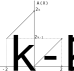
\includegraphics[width=0.9\textwidth]{doplnek-graf.pdf}
\end{column}
\hfill
\begin{column}{0.5\textwidth}
\begin{tabular}{|c|c|}\hline
{\small Binární hodnota}  & {\small Dvojkový doplněk} \\\hline
\textbf{0}0000000 & $0_{(10)}$ \\ \hline
\textbf{0}0000001 & $1_{(10)}$ \\ \hline
... & ... \\\hline
\textbf{0}1111110 & $126_{(10)}$ \\ \hline
\textbf{0}1111111 & $127_{(10)}$ \\ \hline
\textbf{1}0000000 & $-128_{(10)}$ \\ \hline
\textbf{1}0000001 & $-127_{(10)}$ \\ \hline
\textbf{1}0000010 & $-126_{(10)}$ \\ \hline
... & ... \\\hline
\textbf{1}1111101 & $-3_{(10)}$ \\ \hline
\textbf{1}1111110 & $-2_{(10)}$ \\ \hline
\textbf{1}1111111 & $-1_{(10)}$ \\ \hline
\end{tabular}
\end{column}
\end{columns}
\end{frame}

\begin{frame}
\frametitle{Opačné číslo}
\begin{itemize}
\item Protože sčítání funguje s dvojkovým doplňkem, tak nemusíme navrhovat obvod pro odčítání, jednoduše \texttt{A-B} vypočteme jako \texttt{A+(-B)}
\item potřebujeme vymyslet jak získat z \texttt{B} hodnotu \texttt{-B}
\begin{itemize}
\item víme, že záporné $X = 2^k-|X|$
\item pokud znegujeme každý bit, tak je to vlastně $(2^{k-1}-1)-X$, protože $2^{k-1}-1$ je číslo složené z $k$ jedniček
\end{itemize}
\item Výsledný postup je tedy:
\begin{enumerate}
\item znegujte všechny bity čísla $X$
\item k výslednému číslu přičti 1
\end{enumerate}
\end{itemize}

Příklad:\\
\texttt{53=0b00110101} znegováním cifer dostaneme \texttt{-54=0b11001010} po přičtení 1 pak  \texttt{-53=0b11001011}

\end{frame}


\begin{frame}
\frametitle{Odčítání}


\begin{columns}
\begin{column}{0.5\textwidth}
Odčítání lze řešit:
\begin{itemize}
\item speciálním obvodem podobným sčítačce se všemi možnostmi zrychlení jako byly u sčítání
\item nebo z druhého čísla vytvoříme číslo opačné a to pak jednoduše sečteme s tím prvním
\end{itemize}
\end{column}
\hfill
\begin{column}{0.5\textwidth}
\begin{center}
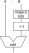
\includegraphics[width=0.5\textwidth]{odcitani.pdf}
\end{center}
\end{column}
\end{columns}


\end{frame}


\begin{frame}
\frametitle{Násobení a dělení}

\begin{itemize}
\item pro násobení lze odvodit, že pokud bychom ignorovali znaménko a spočítali $M\cdot N$, pak pro $M$,$N$ obě k-bitová čísla musíme výsledek upravit takto:
\end{itemize}
$A(M\cdot N) = A(M) \cdot A(N)$\\
\phantom{$A(M\cdot N)$ }$-A(M) \cdot 2^k$ \phantom{xxxxx} pokud $M<0$\\
\phantom{$A(M\cdot N)$ }$-A(N) \cdot 2^k$ \phantom{xxxxx} pokud $N<0$
%\begin{itemize}
\begin{itemize}
\item protože reprezentace záporného čísla dvojkovým doplňkem je vlastně $A(M) = 2^k+M$, pak součin dvou záporných čísel je $(2^k+M)\cdot (2^k+N) = 2^{2\cdot k}+2^k \cdot M + 2^k \cdot N + M \cdot N$
\end{itemize}
%\end{itemize}
\begin{itemize}
\item moderní násobení a dělení počítá s absolutními hodnotami a nakonec určíme znaménko výsledku podle znaménka operandů.
\begin{itemize}
\item nejvyšší bit značí znaménko
\item výpočet opačného čísla je rychlý a levný
\end{itemize}
\end{itemize}
\end{frame}


\begin{frame}
\frametitle{Čísla se znaménkem}
Reprezentace celých čísel

V jazyce C jsou typy:
\begin{tabular}{|l|r|r|c|}\hline
typ & min & max & počet\\
 &  & &  bajtů\\ \hline
char & -128 & 127 & 1 \\ \hline
short & -32 768 & 32 767 & 2 \\ \hline 
long & -2 147 483 648 & 2 147 483 647 & 4 \\ \hline
long long & -9 223 372 036 & 9 223 372 036  & 8 \\ 
 & \phantom{xx} 854 775 808 & \phantom{xx}854 775 807 &  \\ \hline
\end{tabular}

\begin{itemize}
\item Norma C má ve skutečnosti min o 1 větší , kvůli procesorům s jedničkovým doplňkem -- ten se dnes již prakticky nepoužívá
\item Stejně tak \texttt{int} musíte otestovat, zda je 2 bajtový nebo 4 bajtový
\end{itemize}

\end{frame}


\begin{frame}[fragile, shrink=5]
\frametitle{Kvíz}

Uvažujte tento program:
\begin{minted}{c}
#include <stdio.h>
int main() {
  unsigned char a=150u, b=120u, c;
  char sa=-100, sb=-80, sc;
  
  c=a+b;
  sc=sa+sb;
  printf("c=%u sc=%d\n", c, sc);
}
\end{minted}

Co program vytiskne:
\begin{itemize}
\item[A] c=270 sc=-180
\item[B] c=14 sc=-76
\item[C] c=14 sc=76
\item[D] c=-14 sc=-76
\item[E] Numeric error
\end{itemize}
\end{frame}

\begin{frame}
\frametitle{Přetečení při sčítání čísel bez znaménka}


Pokud se podíváme co se stalo, unsigned char je 8-bitová reprezentace čísel:\\
\texttt{\phantom{x}150 = \phantom{x}1001 0110}\\
\texttt{+120 = \phantom{x}0111 1000}\vspace{-6pt}\\
\rule[0pt]{3.6cm}{0.4pt}\\
\texttt{\phantom{xx}14 = \phantom{x}0000 1110}\\
\texttt{\phantom{x}270 =1 0000 1110}

Protože se výsledek nevejde do 8-bitů, nejvyšší jednička se ztratí a výsledek je pouze 14.

Pokud přetečení chcete detekovat, máte následující možnosti:
\begin{itemize}
\item C23 bool ckd\_add(type1 *result, type2 a, type3 b) -- součet dvou čísel s detekcí přetečení
\item GNU GCC 5+, Clang 3.8+ \_\_builtin\_add\_overflow(a, b, result) -- obě verze i pro sub a mul
\end{itemize}
\end{frame}

\begin{frame}
\frametitle{Přetečení}

Přetečení při sčítání čísel se znaménkem je složitější. Co je dobře a co je špatně:
\bigskip
\begin{columns}
\begin{column}{0.3\textwidth}
\texttt{-112 = 10010000}\\
\texttt{+\phantom{x}45 = 00101101}\\
\vspace{-8pt}
\rule[0pt]{3cm}{0.1pt}\\
\texttt{\phantom{x}-67 = 10111101}\\
\begin{center}
\large DOBŘE
\end{center}
\end{column}
\hfill
\begin{column}{0.3\textwidth}
\texttt{\phantom{xx}-12 = 11110100}\\
\texttt{+ -20 = 11101100}\\
\vspace{-8pt}
\rule[0pt]{3cm}{0.1pt}\\
\texttt{\phantom{xx}-32 =\textcolor{red}{1}11100000}\\
\begin{center}
\large DOBŘE
\end{center}
\end{column}
\hfill
\begin{column}{0.3\textwidth}
\texttt{\phantom{xx}-90 = 10100110}\\
\texttt{+ -42 = 11010110}\\
\vspace{-8pt}
\rule[0pt]{3cm}{0.1pt}\\
\texttt{\phantom{xx}124 =\textcolor{red}{1}01111100}\\
\begin{center}
\large ŠPATNĚ
\end{center}
\end{column}
\end{columns}
\bigskip
\begin{itemize}
\item Přetečení při sčítání čísel se znaménkem nastane právě tehdy, když dojde k přenosu na posledních cifrách a zároveň nedojde k přenosu na předposledních cifrách:
\begin{itemize}
\item overflow = $c_n$ xor $c_{n-1}$; $c_n$ je nejvyšší carry, $c_n$ je druhé nejvyšší carry
\end{itemize}
\item Druhá možnost je sledovat, zda při součtu dvou kladných čísel máme záporná výsledek, nebo při součtu dvou záporných čísel je kladný výsledek:
\begin{itemize}
\item overflow = ($a_n$ and  $b_n$ and (not $s_n$)) or ((not $a_n$) and  (not $b_n$) and $s_n$); $a_n$, $b_n$ jsou nejvyšší bity sčítanců; $s_n$ je největší bit výsledku
\end{itemize}
\end{itemize}
\end{frame}

\begin{frame}
\frametitle{Kvíz}

\begin{center}
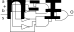
\includegraphics[width=0.6\textwidth]{overflow.pdf}
\end{center}

Při sčítání dvou čísel s odlišnými znaménky:
\begin{itemize}
\item[A] může dojít k přetečení jen v dvojkovém doplňku
\item[B] může dojít k přetečení pouze při jiné reprezentaci než je dvojkový doplněk
\item[C] nemůže dojít pouze při reprezentaci v dvojkovém doplňku
\item[D] nemůže dojít v žádné reprezentaci čísel se znaménkem
\end{itemize}
\end{frame}



\begin{frame}
\frametitle{Jiné reprezentace záporných čísel}

Čísla s posunutou nulou:

\begin{columns}
\begin{column}{0.5\textwidth}
\begin{itemize}
\item pro k-bitovou reprezentaci zvolíme číslo S (většinou $S=2^{k-1}$ nebo $S=2^{k-1}-1$)
\item reprezentace -- kód čísla X je $A(X) = X+S$
\item rozkódování je funkcí $D(A) = A-S$
\item rozsah čísel reprezentovaných je $<-S, 2^{k}-S-1>$
\end{itemize}
\end{column}
\hfill
\begin{column}{0.5\textwidth}
Pro k=8 a S=127
\bigskip
\begin{tabular}{|c|c|}\hline
{\small Binární hodnota}  & {\small Hodnota} \\\hline
00000000 & $-127_{(10)}$ \\ \hline
00000001 & $-126_{(10)}$ \\ \hline
... & ... \\\hline
01111110 & $-1_{(10)}$ \\ \hline
01111111 & $0_{(10)}$ \\ \hline
10000000 & $1_{(10)}$ \\ \hline
10000001 & $2_{(10)}$ \\ \hline
... & ... \\\hline
11111110 & $127_{(10)}$ \\ \hline
11111111 & $128_{(10)}$ \\ \hline
\end{tabular}
\end{column}
\end{columns}

\end{frame}

\begin{frame}
\frametitle{Počítání s posunutou nulou}

\begin{itemize}
\item sčítání a odčítání čísel s posunutou nulou je složitější:
\item $A ( X + Y )=( X + Y )+S =( X + S )+(Y + S ) - S = A ( X )+ A (Y ) -S$
\item $A ( X - Y )=( X - Y )+ S =( X + S ) - (Y +S )+S = A ( X ) - A (Y )+S$
\item násobení je ještě složitější:
\item $A ( X \cdot Y )=( X \cdot Y )+S =( X + S )\cdot(Y + S )-( X + S +Y +S )\cdot S + S^2+ S
= A ( X )\cdot A (Y ) - ( A ( x)+ A ( y ))\cdot S + S^2 +S$
\end{itemize}
\bigskip
\begin{itemize}
\item Přetečení:
\begin{itemize}
\item při sčítání jsou znaménka sčítanců stejná a výsledek má jiné znaménko
\item při odčítání čísel s různými znaménky má výsledek jiné znaménko než menšenec
\end{itemize}
\end{itemize}
\end{frame}


\begin{frame}
\frametitle{Jiné reprezentace záporných čísel}

Doplněk jedné:
\begin{itemize}
\item záporné číslo je negací bitů opačného čísla 
\begin{itemize}
\item pro $X\ge0$ je reprezentace $A(X) = X$
\item pro $X<0$ je reprezentace $A(X) = 2^k-1-|X|$
\end{itemize}
\item nevýhody: dvě reprezentace 0, složitější sčítání čísel se znaménky
\end{itemize}
\bigskip
BCD formát
\begin{itemize}
\item jiná reprezentace celých čísel, každá cifra jeden nibble 
\begin{itemize}
\item číslo \texttt{1234} je uloženo v hexadecimálním tvaru jako \texttt{0x1234}
\end{itemize}
\item výhody: snadný převod na desítkovou soustavu
\item nevýhody: neefektivní reprezentace, složitější počítání
\end{itemize}
\end{frame}


\section{Reálná čísla}


\begin{frame}
\frametitle{Reálná čísla}

\begin{itemize}
\item Celé číslo $X$ v binární soustavě je součet $k$ bitů $b_i$ vynásobených mocninami 2, tedy $ X = \sum_{i=0}^{k-1} b_i 2^{i} $
\item Reálné číslo $X$ v binární soustavě je obdobný součet $k+j$ bitů $b_i$ vynásobených mocninami 2, ale začneme již v záporných mocninách: $X = \sum_{i=-j}^{k} b_i 2^{i}$
\item jistě si všichni pamatujete ze střední školy, že $2^{-j} = \frac{1}{2^j}$
\end{itemize}


\begin{center}
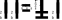
\includegraphics[width=0.65\textwidth]{float_bin.pdf}
\end{center}

\end{frame}


\begin{frame}
\frametitle{Reálná čísla s pevnou desetinnou čárkou}

Čísla s pevnou desetinnou čárkou (fixed point numbers):

\begin{itemize}
\item obdoba čísel s posunutou 0
\item reálné číslo je reprezentované k-bitovým celým číslem se znaménkem, dále zvolíme pevný počet desetinných míst s bitů, kdy $0 \le s \le k$
\item reprezentace -- kód čísla X je $A(X) = \lceil X \cdot 2^s \rceil$
\item rozkódování je funkcí $D(A) = \frac{A}{2^s}$
\item rozsah čísel reprezentovaných je $<-\frac{2^{k-1}}{2^s}, \frac{2^{k-1}-1}{2^s}>$
\item přesnost reprezentace čísel je $\pm \frac{1}{2^s}$.
\end{itemize}

Speciální případ:
\begin{itemize}
\item pokud chcete reprezentovat reálná čísla z intervalu $<0,1)$
\item pak můžete nastavit $s=k$ a použít bezznaménkovou reprezentaci celých čísel
\item dosáhnete lepší přesnosti než odpovídající \texttt{float}, nebo \texttt{double}
\end{itemize}

Některé SIMD instrukce používají pevnou desetinnou čárku.

\end{frame}

\begin{frame}
\frametitle{Reálná čísla s pevnou desetinnou čárkou}

Počítání s čísly s pevnou desetinnou čárkou:

\begin{itemize}
\item součet a rozdíl je součtem a rozdílem celočíselné reprezentace čísel
\item násobení je složitější:
\begin{itemize}
\item $A(X \cdot Y) = (X \cdot Y ) \cdot 2^s = \frac{(X \cdot 2^s)\cdot( Y\cdot 2^s) }{2^s} = \frac{A(X) \cdot A(Y)}{2^s}$
\end{itemize}
\item dělení je obdobné:
\begin{itemize}
\item $A(\frac{X}{Y}) = (\frac{X}{Y}) \cdot 2^s = \frac{(X \cdot 2^s)\cdot2^s }{( Y\cdot 2^s)} = \frac{A(X) \cdot 2^s}{A(Y)}$
\end{itemize}
\item Nejedná se o výrazné zesložitění, protože násobení číslem $2^s$ je posun o s bitů doleva a dělení číslem $2^s$ je posun o s bitů doprava.
\end{itemize}



\end{frame}


\begin{frame}
\frametitle{Plovoucí desetinná čárka}

Plovoucí desetinná čárka (floating point numbers)

\bigskip

Obdoba vědeckého zápisu reálných čísel:
$-123 000 000 000 000.0 = -1.23 \cdot 10^{14} = -1.23\text{E} 14$\\
$0.000 000 000 000 123 = -1.23 \cdot 10^{-13} = -1.23\text{E}-13$\\

\bigskip

Binární reprezentace používá obdobně mocninu 2:\\
$110 1100 0000 0000.0 = 1.1011 \cdot 2^{14} = 1.1011\text{E} 14 = 29696_{10}$\\
$-0.0000 0000 0000 0001 1101 = -1.1101 \cdot 2^{-16} = -1.1101\text{E}-16 \approx$\\
\phantom{xxxxxxxxxxxxxxxxxxxxxxxxxxxxxxxxxxxxxxxxxx}$\approx0.00002765_{10}$\\

\bigskip

Všimněte si, že každé reálné číslo (kromě 0) začíná v binárním vědeckém zápisu jedničkou.


\end{frame}

\begin{frame}
\frametitle{IEEE-754}

Standard IEEE-754 definuje, jakým způsobem zakódovat reálné číslo do 32, 64 bitů.

Reálné 32-bitové číslo obsahuje:
\begin{itemize}
\item 1 bit znaménko (pozn. existuje 0 i -0)
\item 8 bit hodnota exponentu s posunutou nulou o 127
\item 23 bitů hodnota mantisy, tedy cifer reprezentujících hodnotu
\end{itemize}
\bigskip
Reálné 64-bitové číslo obsahuje:
\begin{itemize}
\item 1 bit znaménko (pozn. existuje 0 i -0)
\item 11 bitů hodnota exponentu s posunutou nulou o 1023
\item 23 bitů hodnota mantisy, tedy cifer reprezentujících hodnotu
\end{itemize}

\end{frame}


\begin{frame}
\frametitle{IEEE-754}

Příklad:
Reálné číslo $0.828125_{(10)} = 0.5+0.25+0.0625+0.015625=2^{-1}+2^{-2}+2^{-4}+2^{-6} = 0.110101_{(2)}$.\\
Číslo převedeme do vědecké notace: $0.110101 = 1.10101\text{E}-1$.\\
Exponent $e=-1$, reprezentace s posunutou nulou o 127 je $A(-1)=-1+127 = 126$.\\
Abychom neplýtvali zbytečně bity, pro normalizovaná čísla se první 1 mantisy neukládá do binární reprezentace čísla:

\begin{center}
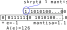
\includegraphics[width=0.4\textwidth]{float_priklad.pdf}
\end{center}

Zkuste si \url{https://www.h-schmidt.net/FloatConverter/IEEE754.html}
\end{frame}

\begin{frame}
\frametitle{IEEE-754}

Normalizované číslo, je každé číslo, které lze zapsat jako \texttt{1.XXXXX E exp}, kde exp je číslo od -126 do 127, tedy jehož reprezentace je od 1 do 254.

\bigskip
Denormalizovaná čísla jsou čísla, která lze zapsat jako \texttt{0.XXXXX E -126}, tedy například 0.0, nebo všechna čísla v intervalu $(-1.17549\text{E}-38,1.17549\text{E}-38)$, tedy od $(-2^{-126},2^{-126})$.

\bigskip
Pokud je reprezentace exponentu nastavena na samé 1, tedy 255, tzn. hodnota exponentu je 128, pak se jedná o speciální čísla. 
\begin{itemize}
\item pokud je mantisa 0, pak se jedná o nekonečno, podle znaménka \textit{-inf}, nebo \textit{inf}.
\item pokud je mantisa nenulová, pak se jedná o speciální výraz \textit{NaN} -- Not a Number, tedy chybná hodnota čísla, například po výpočtu odmocniny záporného čísla 
\end{itemize}
\end{frame}

\begin{frame}[shrink=5]
\frametitle{IEEE-754}

Přehled reálných čísel:
\begin{tabular}{|c|c|l|}\hline
Exponent & Mantisa &  Hodnota \\ \hline
00000000 & 0 &  0.0 -- čistá nula \\ \hline
00000000 & nenulová &  Denormalizovaná čísla blízká 0 \\ \hline
00000001 & 0 &  nejmenší normalizované číslo se skrytou 1 v mantise \\ \hline
\small 1 až 254 & cokoliv &  normalizovaná čísla, skrytá 1 v mantise \\ \hline
11111111 & 0 &  nekonečno \\ \hline
11111111 & nenulová &  NaN chybná hodnota \\ \hline
\end{tabular}
\bigskip

Denormalizované číslo s nejmenší absolutní hodnotou různé od 0 je:
\begin{itemize}
\item \small exponent = 0 (-126), mantisa=000...0001, hodnota = $2^{-23+(-126)} \approx 1.4\text{E}-45$
\end{itemize}
Normalizované číslo s nejmenší absolutní hodnotou:
\begin{itemize}
\item \small exponent = 1 (-126), mantisa=000...0000, hodnota = $2^{-126} \approx 1.17\text{E}-38$
\end{itemize}
Normalizované číslo s největší absolutní hodnotou:
\begin{itemize}
\item \small exponent = 255 (127), mantisa=111...1111, hodnota = $(2-2^{-23})2^{127} \approx 3.4\text{E}38$
\end{itemize}
\end{frame}


\begin{frame}
\frametitle{IEEE-754 revize 2008 }

Standard IEEE-754 navíc definuje reálné číslo s 16 bity (half precision) a s 128 bity (quad precision).

Reálné 16-bitové číslo obsahuje:
\begin{itemize}
\item 1 bit znaménko 
\item 5 bitů hodnota exponentu s posunutou nulou o 15
\item 10 bitů hodnota mantisy, (plus 11tý bit skrytý neukládaný)
\end{itemize}
\bigskip
Reálné 128-bitové číslo obsahuje:
\begin{itemize}
\item 1 bit znaménko 
\item 15 bitů hodnota exponentu s posunutou nulou o 16383
\item 112 bitů hodnota mantisy, (plus 113 bit skrytý)
\end{itemize}

\end{frame}


\begin{frame}
\frametitle{IEEE-754 }

Porovnání reálných čísel na velikost:
\begin{itemize}
\item Kladná čísla jsou vždy větší než záporná
\item Po odstranění znamének, lze absolutní hodnoty čísel porovnat tak, jak jsou uložené v paměti jako celé číslo bez znaménka
\begin{itemize}
\item To je možné díky zvolené reprezentaci exponentu jako čísla s posunutou nulou
\item Větší exponent větší číslo, při rovnosti exponentů větší mantisa znamená větší číslo
\end{itemize}
\end{itemize}
\end{frame}


\begin{frame}
\frametitle{IEEE-754}

Sčítání nebo odčítání dvou reálných čísel ve vědecké notaci
\begin{enumerate}
\item Převést mantisy čísel na společný exponent, který má hodnotu největšího exponentu (porušíme notaci)
\item Provést součet, nebo rozdíl mantis i se skrytými jedničkami
\item Výsledné číslo normalizovat
\begin{itemize}
\item při sčítání se může exponent zvětšit
\item při odčítání se exponent může zmenšit
\end{itemize}
\end{enumerate}

\end{frame}


\begin{frame}
\frametitle{IEEE-754}

Příklad: Sčítání dvou reálných čísel 31.5+0.75

$31.5_{(10)} = 11111.1_{(2)} = 1.11111\text{E}4$ \phantom{xxx} $0.75_{(10)} = 0.11_{(2)} = 1.1\text{E}-1$

\bigskip
Obě čísla převedeme na stejný exponent 4 a sečteme:\\
\texttt{\phantom{xx}1.11111}\\
\texttt{\phantom{xx}0.000011}\vspace{-6pt}\\
\rule[0pt]{2cm}{0.4pt}\\
\texttt{\phantom{x}10.000001}\\

Výsledné číslo musíme znormalizovat zvýšením exponentu na 5 a tím posunutím desetinné čárky vlevo:\\
$10.000001\text{E}4 = 1.0000001\text{E}5$\\

Toto číslo je reprezentací čísla 32.25.

\end{frame}

\begin{frame}
\frametitle{IEEE-754 -- Násobení}

Násobení dvou reálných čísel:
\begin{enumerate}
\item Exponent výsledku je součet exponentů čísel
\item Mantisa výsledku je součin mantis čísel (i se skrytými jedničkami)
\item Výsledné číslo normalizovat
\begin{itemize}
\item podle výsledku násobení mantis je někdy nutné zvýšit exponent o 1 a vyrotovat mantisu doprava
\end{itemize}
\end{enumerate}
\end{frame}

\begin{frame}
\frametitle{IEEE-754 -- Násobení}

Příklad: Vynásobíme čísla $0.375 \cdot 1.5$

$0.375_{(10)} = 0.011_{(2)} = 1.1\text{E}-2$ \phantom{xxx} $1.5_{(10)} = 1.1_{(2)} = 1.1\text{E}0$

Součin mantis je:\\
\texttt{\phantom{xxx}11} odpovídá \texttt{1.1}\\
\texttt{\phantom{xx}*11} odpovídá \texttt{1.1}\vspace{-6pt}\\
\rule[0pt]{2cm}{0.4pt}\\
\texttt{\phantom{xxx}11}\\
\texttt{\phantom{xx}11}\vspace{-6pt}\\
\rule[0pt]{2cm}{0.4pt}\\
\texttt{\phantom{x}1001} odpovídá \texttt{10.01} protože výsledek má dvě desetinná čísla

Exponent vychází $-2+0=-2$, ale výsledek součinu mantis potřebujeme normalizovat, neboli zvětšit exponent o 1 na $-1$.

Tím dostáváme výsledek $10.01\text{E}-2 = 1.001\text{E}-1$ což je správný výsledek $0.5625_{(10)}$

\end{frame}

\begin{frame}[fragile]
\frametitle{IEEE-754}

Reálná čísla shrnutí:
\begin{itemize}
\item reálná čísla s plovoucí čárkou umí reprezentovat čísla ve velmi velkém rozsahu:
\begin{itemize}
\item float -- absolutní hodnota čísel od $1.175494351\text{E}-38$ do $3.402823466\text{E} + 38$
\item double -- absolutní hodnota čísel od $2.2250738585072014\text{E} - 308$ do $1.7976931348623158\text{E} + 308$
\end{itemize}
\item přesnost čísla se udává na počet validních cifer:
\begin{itemize}
\item float -- v desítkové soustavě 6-7 platných cifer
\item double -- v desítkové soustavě 15-16 platných cifer
\end{itemize}
\end{itemize}

POZOR: Následující \texttt{while} cyklus neskončí:
\begin{minted}{c}
  float a=1.0, step=5e-8;
  while (a*a<1.01) {
    a+=step;
  }
\end{minted}
\end{frame}


\begin{frame}
\frametitle{Bonusový bod}

Kvíz s bonusovou otázkou za tuto hodinu.

\end{frame}


\end{document}

